%%%%%%%%%%%%%%%%%%%%%%%%%%%%%%%%%%%%%%%%%%%%%%%%%%%%%%%
%% Unofficial class for ANR Project proposals
%%
%% v1.2.4 - 21/02/2023: updated content to match the 2023 version of the ANR template, thanks to Vincent Colotte.
%% v1.2.3 - 08/09/2021: adjusted footer and header, thanks to Adel Noureddine.
%% v1.2.2 - 21/11/2020: adjusted to allow lists in notes, thanks to Christophe Gravier.
%% v1.2.1 - 25/02/2020: modification to fit the changes in packages pgfgantt, thanks to Nicolas Marchand.
%% v1.2   - 02/03/2019: minor adjustments to match the 2019 version of the template.
%% v1.1   - 12/04/2018: minor adjustments in the class file.
%% v1     - 07/03/2018: first draft.
%%
%% Vincent Labatut 2018-23 
%% <vincent.labatut@univ-avignon.fr>
%% https://www.overleaf.com/latex/templates/unofficial-template-for-anr-proposals/yqgzsxkzrqkw
%% Creative Commons CC BY 4.0
%%
%% Please tell me if you find any error.
%% And if you use this model for your ANR project: 
%% I only take 8% of your accepted budget ;)
%%%%%%%%%%%%%%%%%%%%%%%%%%%%%%%%%%%%%%%%%%%%%%%%%%%%%%%
\documentclass{anr/proposal}





%%%%%%%%%%%%%%%%%%%%%%%%%%%%%%%%%%%%%%%%%%%%%%%%%%
% Search for "NOTE:" to get to the parameters worth adjusting to your needs
% There are some such NOTEs in the anr/proposal.cls file, too.
%%%%%%%%%%%%%%%%%%%%%%%%%%%%%%%%%%%%%%%%%%%%%%%%%%






%%%%%%%%%%%%%%%%%%%%%%%%%%%%%%%%%%%%%%%%%%%%%%%%%%
% project details
\acronym				        % acronym of the project
	{\textsc{SPACE2050}}
\committee				        % scientific evaluation committee (CES)
	{PEPR Ville Durable et Bâtiment Innovant}
\instrument{PEPR VDBI}		        % funding instrument
\acyear{2023}			        % academic year of the call
\title                          % full title of the project
    {\myacronym{}: Pour une approche Systémique de la Planification bAs Carbone des tErritoires}
\subtitle                           % subtitle of the project (optional)
    {Scénarios, actions et évaluations}
\investigator{Alain L'Hostis} % principal investigator
\duration{36 months}            % duration of the project
\funding{3 M\euro}          % requested funding
% NOTE: all the above fields must be filled (except the subtitle which is optional)
% NOTE: use command \myxxxxx{} to mention information xxxx in the text, e.g. \myacronym{}


%%%%%%%%%%%%%%%%%%%%%%%%%%%%%%%%%%%%%%%%%%%%%%%%%%
% bibliography
\addbibresource{anr_biblio.bib}
\addbibresource{zotero_ALH.bib}
% NOTE: look for "bibliographic settings" in the class if you want to 
% change the formatting of the bibliography (e.g. switch to author-year instead of numeric)


% make bold names of authors of the consortium
\ExecuteBibliographyOptions{maxnames=99,giveninits}
\DeclareNameAlias{default}{family-given/given-family}
\forcsvlist{\listadd\boldnames}
  {{Kilani, Moez}, {Kilani, M.}, {Kilani, M\bibinitperiod}}
\forcsvlist{\listadd\boldnames}
  {{Zerguini, Seghir}, {Zerguini, Z.}, {Zerguini, Z\bibinitperiod}}


\setlength{\parindent}{0pt}
\setlength{\parskip}{\baselineskip}



%%%%%%%%%%%%%%%%%%%%%%%%%%%%%%%%%%%%%%%%%%%%%%%%%%
% partners
\newcommand{\colUGE}[1]{\textcolor{partnercol1}{#1}}
\newcommand{\colEFF}[1]{\textcolor{partnercol2}{#1}}
\newcommand{\colINR}[1]{\textcolor{partnercol3}{#1}}
\newcommand{\colUT}[1]{\textcolor{partnercol4}{#1}}
\newcommand{\colTUT}[1]{\textcolor{partnercol5}{#1}}
% NOTE: colors go from partnercol1 to partnercol8
% if you need more colors, add them in the class file, look for "color settings"


%%%%%%%%%%%%%%%%%%%%%%%%%%%%%%%%%%%%%%%%%%%%%%%%%%
% work packages
% NOTE: WP are defined using the \wpdef{label}{Title} macro. 
% NOTE: Cross-referencing works as usual, with the \ref{label} macro.
% NOTE: WPs are numbered from 0. If you want to start from 1, look for "work packages and tasks" 
% in the class file (anr.cls), and read the note there.


%%%%%%%%%%%%%%%%%%%%%%%%%%%%%%%%%%%%%%%%%%%%%%%%%%
% tasks
% NOTE: tasks are defined using the \tdef{label}{Title} macro. 
% NOTE: Cross-referencing works as usual, with the \ref{label} macro.


%%%%%%%%%%%%%%%%%%%%%%%%%%%%%%%%%%%%%%%%%%%%%%%%%%
% writer comments
\usepackage%[disable]	% uncomment to hide all the notes
	{todonotes} 
\newcommand{\noteANR}[1]{\todo[color=gray!100, author=\textbf{ANR}, inline, caption={}]{#1}}
\newcommand{\notePEPR}[1]{\todo[color=gray!40, author=\textbf{PEPR}, inline, caption={}]{#1}}
\newcommand{\noteSM}[1]{\todo[color=red!40, author=\textbf{Stéphanie}, inline, caption={}]{#1}}
\newcommand{\noteJZ}[1]{\todo[color=green!40, author=\textbf{Jing}, inline, caption={}]{#1}}
\newcommand{\noteRM}[1]{\todo[color=blue!40, author=\textbf{Richard}, inline, caption={}]{#1}}
% NOTE: you can setup other writers by pasting and editing the above lines


\begin{document}
\maketitle




%%%%%%%%%%%%%%%%%%%%%%%%%%%%%%%%%%%%%%%%%%%%%%%%%%
%%%%%%%%%%%%%%%%%%%%%%%%%%%%%%%%%%%%%%%%%%%%%%%%%%
%%%%%%%%%%%%%%%%%%%%%%%%%%%%%%%%%%%%%%%%%%%%%%%%%%
%%%%%%%%%%%%%%%%%%%%%%%%%%%%%%%%%%%%%%%%%%%%%%%%%%




%%%%%%%%%%%%%%%%%%%%%%%%%%%%%%%%%%%%%%%%%%%%%%%%%%
% consortium
\begin{center}
	\textbf{Consortium:} 
	\colUGE{LVMT (Univ Eiffel)}, 
	\colEFF{Efficacity},
	\colINR{LMD (INR)},
	\colUT{CGCS (UT)},
	\colTUT{FI (TUT)}
\end{center}




%%%%%%%%%%%%%%%%%%%%%%%%%%%%%%%%%%%%%%%%%%%%%%%%%%
% general comments

\notePEPR{\textit{Le dossier ci-dessous }\textit{\textbf{doit être de 20 pages maximums pour les sections de 1 à 8. }}

\textit{\textbf{La section Annexes (Annexe Partenariats et Annexe Publications) ne doit pas dépasser les 10 pages. }}

\textit{\textbf{Le dossier doit être rédigé en }}\textit{\textbf{police Arial 11pt, interligne 1,15, }}\textit{\textbf{de préférence en anglais}}\textit{\textbf{. }}\textit{Les informations précises demandées au-dessus de ce cadre ne sont pas décomptées dans le nombre de pages.} \textit{Toutes les consignes écrites en violet devront être éliminées par les rédacteurs du projet.}
}


\begin{spacing}{0.1}
\tableofcontents
\end{spacing}
%%%%%%%%%%%%%%%%%%%%%%%%%%%%%%%%%%%%%%%%%%%%%%%%%%
% project summary
%%%%%%%%%%%%%%%%%%%%%%%%%%%%%%%%%%%%%%%%%%%%%%%%%%
% project summary
\phantomsection
\addcontentsline{toc}{section}{Summary}

{	\vspace{0.2cm}
	\centering
    \small
    \begin{table}
        \centering
        \begin{tabular}{p{0.30\textwidth} p{0.60\linewidth}ll}
        	\hline
             Acronym& \textbf{\myacronym} & &\\
             \hline
             Titre du projet en français& \textbf{\mytitle{}} & &\\
             \hline
             Titre du projet en anglais& \textbf{} & &\\
             \hline
             Keywords/Mots-clefs \newline (min 5-max 10)&  \textbf{} & &\\
             \hline
             Leading institution /Établissement porteur& \textbf{Université Gustave Eiffel} & &\\
             \hline
             Défi principal choisi&  & &\\ 
             \hline
             Autre défis que le défi principal& & &\\
             \hline
             Scientific coordinator& \textbf{Alain L'Hostis}& &\\
             \hline
             Project duration& & &\\
             \hline
             Requested funding& & &\\
             \hline
        \end{tabular}
        \label{tab:my_label}
    \end{table}
 }   

Partner institution(s) involved in the project/Liste des établissements du consortium :

{	\vspace{0.2cm}
	\centering
    \small
    \begin{table}
        \centering
        \begin{tabular}{p{0.50\textwidth} p{0.50\linewidth}}
        	\hline
             Name of the institutions of higher education and research / Établissements d’enseignement supérieur et de recherche& Activity / Secteur(s) d’activité\\  \hline
            \colUGE{Université Gustave Eiffel }& Higher education and research	\\        \hline 
             \colEFF{Efficacity}&  Research and development		\\        \hline
             &  \\		      \hline
             & \\             \hline
             &  \\
     & \\
     & \\
     & \\
     & \\
        \end{tabular}
        
        \label{tab:my_label}
    \end{table}
}

%%%%%%%%%%%%%%%%%%%%%%%%

\iffalse  % for commenting
% summary table
\subsectionn{Summary table of persons involved in the project}


{	\vspace{0.2cm}
	\centering
    \small
	\begin{tabular}{p{0.13\textwidth} p{0.13\linewidth} p{0.13\linewidth} p{0.10\linewidth} p{0.22\linewidth} p{0.13\linewidth}}
		\hline
        \rowcolor{headcolor!20}
	    \textbf{Partner} & \textbf{Last name} & \textbf{First name} & \textbf{Current \newline position} & \textbf{Role \& \newline responsibilities} & \textbf{Involvement \newline (pers.month)} \\
		\hline
		\colUGE{Université Gustave Eiffel}& L'Hostis& Alain& DR& Coordinator \newline Leads WP \ref{wp:ProjMgt} \newline Inv. Tasks \ref{tsk:DataOT}, \ref{tsk:ClassifFT}, \ref{tsk:ExpYT} & 36 p.m \\
		\hline
        \colUGE{Université Gustave Eiffel}& Bonin& Olivier& PR & Leads WP \ref{wp:Data} \newline Inv. Tasks \ref{tsk:DataST}, \ref{tsk:DataOT}, \ref{tsk:DataLT} & 18 p.m \\
		\hline
		\colEFF{Efficacity}& Laterrasse& Jean& PR& Leads WP \ref{wp:Classif} \newline Inv. Tasks \ref{tsk:ClassifAT}, \ref{tsk:ClassifYT} & 18 p.m \\
		\hline
		\colEFF{Efficacity}& Wendeln& Matthew& & Leads WP \ref{wp:Exp} \newline Inv. Tasks \ref{tsk:ClassifFT}, \ref{tsk:ExpTT} & 12 p.m \\
		\hline
        & & & & & \\
		\hline
		& & & & & \\
		\hline
	\end{tabular}
}

\fi

%%%%%%%%%%%%%%%%%%%%%%%%


\textit{\mytitle{}} is a \myinstrument{} project led by \myinvestigator{} and submitted to \mycommittee{} in \myacyear{}. It will last for \myduration{}, so we ask for no less than \myfunding{} in order to fund it.






%%%%%%%%%%%%%%%%%%%%%%%%%%%%%%%%%%%%%%%%%%%%%%%%%%
% Context and objectives
%%%%%%%%%%%%%%%%%%%%%%%%%%%%%%%%%%%%%%%%%%%%%%%%%%
% Context and objectives
\section{Context, objectives and previous achievements}

\textit{\textbf{Enjeu opérationnel}} : fournir aux agglos des outils d’aide à la décision fiables pour l’élaboration des PCAET, sachant que les émissions qu’elles génèrent représentent environ 2/3 des émissions. Ces outils doivent en particulier répondre à 2 objectifs : permettre aux agglos de contrôler autant que faire se peut leur trajectoire d’émission




%%%%%%%%%%%%%%%%%%%%%%%%
\subsection{Context, objectives and innovative features of the project
}

\notePEPR{Présenter les enjeux scientifiques, les questions de recherche et définir les objectifs du projet et sa pertinence au regard du cadrage général du PEPR.}
\notePEPR{Présenter l’état de l’art national et international en décrivant la pertinence du positionnement scientifique du projet par rapport aux connaissances actuelles. Décrire les principales hypothèses de travail et les principaux choix réalisés.}



\subsection{Main previous achievements}
\notePEPR{Donner les principales réalisations antérieures par les équipes partenaires, démontrer la qualité des résultats déjà acquis soutenant les hypothèses de recherche et les choix réalisés. Ces éléments doivent notamment permettre d’évaluer l’excellence de la recherche et la crédibilité du projet.}

Modelling drivers and instruments:
\begin{itemize}
    \item Modelling low traffic zones in microsimulation \cite{yinEvaluationLowTrafficNeighborhoods2023}
    \item Modelling TOD scenarios \cite{liuTransportLandUse2014, feudoHowBuildAlternative2014}
\end{itemize}

Modelling rupture scenarios:
\begin{itemize}
    \item Implementing rupture scenario in microsimulation approach \cite{kilaniEnvironmentalImpactsBicycling2023}.
\end{itemize}

Modelling the interfaces:
\begin{itemize}
    \item Modelling the interaction between transport and housing markets \cite{kilaniModelEvaluationUrban2023}.
    \item Land-Use and Transport Interaction model implementation \cite{liuTransportLandUse2014, feudoHowBuildAlternative2014}
    \item Modelling transport and health interaction \cite{manoutAssessingRoleDaily2021}

\end{itemize}


\section{Detailed project description}

\subsection{Project outline, scientific strategy}
\notePEPR{Décrire le défi scientifique relevé par le projet.}
\notePEPR{Donner la vision scientifique globale du projet, son caractère original et ambitieux, ainsi que les implications au regard des objectifs du PEPR.}
\notePEPR{Préciser les formes de rassemblement et d’organisation des forces de recherche.}

\subsubsection{First Challenge: Identifying and assessing the contribution of the main drivers for decarbonising territories}

\textbf{Questions à la recherche :} La plupart des outils d’évaluation des gisements, leviers et actions de décarbonation d’un territoire1 actuellement utilisés dans la planification territoriale fonctionnent selon une approche relativement standardisée : on calcule la production d’objectifs opérationnels à réaliser (par exemple : rénover X logements par an), à partir un catalogue d’actions sectorielles et une évaluation d’impacts par ratios statistiques (parfois complétée par des hypothèses issues d’études ou modèles sectoriels). 

Cette approche a le mérite de fournir aux collectivités une vision d’ensemble des leviers de décarbonation sur leur territoire, de « l’effort climatique à viser » et des ordres de grandeur pour l’accélération nécessaire des principales politiques publiques opérationnelles. 

Cependant elle présente de nombreuses limites :
\begin{itemize}
    \item Les évaluations des potentiels et impacts manquent généralement de finesse et de robustesse.
    \item Les évaluations portent sur des objectifs à atteindre. Or, il s’avère difficile de relier l’évaluation des objectifs (approche « macro ») à une véritable évaluation des actions opérationnelles réellement menées ou envisagées. 
    \item Les outils modélisent les gains GES visés, pas les freins ou les impacts non-désirables probables. Or, les nombreux leviers d’action sont ambivalents : les nouvelles technologies peuvent à la fois permettre d’éviter des déplacements et en générer de nouveaux, des incitations économiques peuvent à la fois orienter les comportements vers des pratiques moins coûteuses en énergie et inciter à une surconsommation, par effet rebond.
    \item Plusieurs leviers et freins clés se trouvent soit écartés de l’évaluation, soit abordés marginalement : 
    \begin{itemize}
        \item Les leviers liés à l’organisation spatiale du territoire, à l’usage du sol et aux disponibilités foncières
        \item Les leviers et freins intersectoriels.
        \item Les flux énergétiques et les capacités des systèmes énergétiques, actuels et futurs (y compris nouveaux systèmes innovants)
    \item Les leviers financiers et comportementaux.
    \end{itemize}
\end{itemize}

Les travaux conduits dans \myacronym   devront permettre d’identifier et d’évaluer les principaux leviers d’action, de définir sous quelles conditions ils peuvent être efficaces, de les hiérarchiser en fonction de l’importance de leurs effets sur les émissions et d’améliorer les estimations d’impact chiffrées à différentes échelles. 

Il paraît a priori possible / souhaitable d’agréger les leviers d’action par grandes catégories sectorielles ou plurisectorielles communiquant entre elles (usage du sol, mobilités, bâtiment, systèmes énergétiques), complétés par une réflexion transverse sur des leviers et verrous actuellement difficiles à évaluer dans l’ensemble des secteurs (incitations économiques, nouvelles technologies…).

Urban models describe the spatial and urban configuration of human activities and their interactions. They can express undesired, unsustainable configurations, but can also serve as ideals and targets to guide the action on territories in a strategic, prospective view. As a counter-proposal to the unsustainable urban model of automobile based urban sprawl, Calthorpe formulated the Transit Oriented Development idea \cite{calthorpeNextAmericanMetropolis1993}. More recently, in the same vein, Moreno enunciated the principle of the 15-minute city as an urban model based on proximity \cite{morenoIntroducing15MinuteCity2021}.

We will test urban models as inputs to create scenarios, and we will assess their impact on key parameters of sustainability.  For instance, TOD scenarios will be used to leverage the potential for urban transformations contained in the ambitious (SEM) regional rail projects in French agglomerations.

\textit{\textbf{Enjeux opérationnels }}: être en capacité dans une approche pré-modélisatrice transversale par rapport aux différents secteurs urbains (bâtiment, mobilité, énergie, aménagement / urbanisme) de prendre en considération de manière cohérente les leviers d’action de même importance. Élaborer de cette façon un modèle simplifié qui pourra être ensuite enrichi par sophistication progressive. Associer des indicateurs de suivi aux leviers d’action retenus.

\subsubsection{Second Challenge: Data, in the light of climate change}

\textit{\textbf{Questions à la recherche}}\textbf{ :} Les démarches de planification classiques s’appuient essentiellement sur l’extrapolation de séries statistiques consolidées aux échelles nationale et régionale\footnote{En France, chaque région est dotée d’un Observatoire régional énergie-climat, référence pour les données utilisées dans la planification bas-carbone transverse (Plan climat, schéma directeur des énergies).} , complétée par des données issues de modèles (climatiques, énergétiques et transports notamment) et des données collectées par la collectivité.  

Ces démarches se heurtent aujourd’hui à plusieurs difficultés majeures : 
\begin{itemize}
    \item Une incapacité à alimenter des scénarios de rupture. Le changement climatique introduit des ruptures qui entachent sérieusement la pertinence de l’utilisation de ces séries statistiques, notamment pour ce qui est de leur profondeur temporelle. Sans renoncer complètement à l’utilisation des séries statistiques, il convient de faire appel au moins de manière complémentaire à d’autres méthodes : approches probabilistes, préférences déclarées, IA…). 
    \item L’éparpillement et l’hétérogénéité des sources de données, le manque de finesse des données utilisées pour les exercices de planification à grande échelle (plan climat, documents stratégiques pour la rénovation des logements sur un territoire…) et des donnes parfois très fines issues d’études ou de modèles.
    \item La difficulté de renouveler rapidement et régulièrement la donnée nécessaire à la planification et au pilotage des plans d’action.
\end{itemize}

\textit{\textbf{Enjeux opérationnels :}} être en capacité de formuler et d’évaluer des scénarios de rupture, donner une profondeur temporelle aux méthodes et outils d’aide à la décision qui seront in fine proposés.  

\subsubsection{Third Challenge: Methods and modelling tools}

\textit{\textbf{Questions à la recherche}}: assembler dans une méthode d’évaluation cohérente et intersectorielle l’ensemble des éléments précédemment établis, et réunir ou développer les modèles et données nécessaires à sa réalisation. Il conviendra notamment de préciser les interactions entre secteurs pris en compte. Une approche de type « land use » peut s’avérer pertinente. Elle suppose notamment qu’y soit intégré par rapport aux approches classiques le secteur énergie (non seulement prise en compte des consos d’énergie dans les bâtiments et les transports, mais aussi de la concurrence dans l’occupation des sols entre les EnR\&R et l’aménagement (bâtiments et infrastructures). En outre, les méthodes et outils proposés devront permettre de reconstituer la dynamique des processus générés par les actions conduites (par exemple, une politique en faveur de la diffusion des véhicules électriques va se traduire dans un premier temps par une augmentation des GES du fait de l’énergie grise consommée par la fabrication des batteries avant de produire des effets bénéfiques, dont l’horizon dépend du type de VE produits…).

 \textit{\textbf{Enjeux opérationnels}}\textbf{ : }reconstituer les trajectoires d’émission des territoires pour différents scénarios et plans d’action associés dans une démarche d’aide à la décision.

 
\subsubsection{Fourth challenge: favoriser une recherche scientifique « tirée par l’aval », qui contribue à alimenter les outils d’aide à la décision des collectivités territoriales}

\textbf{Questions à la recherche}: Il y a actuellement une difficulté réciproque pour (1) mobiliser les méthodes et outils issus de la recherche dans le monde opérationnel et (2) alimenter les laboratoires en expression de besoins, cas d’usage concrets et données des collectivités territoriales. L’expérimentation des outils académiques sur un territoire et la mise à disposition des résultats des recherches (open source) ne suffisent pas pour créer cette passerelle indispensable, et mutuellement bénéfique, entre le monde opérationnel et le monde de la recherche. En effet, il existe de nombreux décalages à combler en matière de cas d’usage traités, de présentation des leviers, indicateurs et résultats, ou encore d’écosystème d’outils et données utilisés par les chercheurs et le monde de l’ingénierie territoriale.  

\textbf{Enjeux opérationnels }: À toutes les étapes du projet, croiser les besoins, les méthodes et les outils des collectivités et des chercheurs. Travailler sur les points d’articulation et de passerelles entre des outils et approches de différents niveaux de sophistication. Intégrer les résultats de la recherche dans des outils opérationnels existants ou à développer, notamment la plateforme prévue dans le projet « PLANETE » (LVMT / Efficacity).  

%%%%%%%%%%%%%%%%%%%%%%%%

\subsection{Scientific and technical description of the project}

\notePEPR{Décrire les objectifs scientifiques du projet et la façon dont ces objectifs seront atteints.}
\notePEPR{Présenter les objectifs intermédiaires, les résultats attendus, l’implication des différents partenaires, leurs différentes responsabilités.}
\notePEPR{Préciser les disciplines impliquées dans le projet (selon les disciplines et sous-disciplines HCERES) ainsi que leur rôle dans la réalisation des objectifs.}
\notePEPR{Présenter la cohérence scientifique du projet et de la pluralité scientifique et la crédibilité des jalons proposés, en justifiant les choix méthodologiques, les technologies et éventuellement les infrastructures de recherche utilisées.}
\notePEPR{Décrire les complémentarités des établissements impliqués.}
\notePEPR{Indiquer l’articulation avec d’autres projets, internes ou/et externes au PEPR.}

%%%
\subsubsection{Leviers d'action et interfaces }
\textbf{Leader: \colEFF{J. Laterrasse}}

The bibliography is handled using \textit{BibLaTeX} and \textit{Biber}\footnote{\url{https://en.wikipedia.org/wiki/Biber_(LaTeX)}} instead of \textit{BibTex}, so no problems with diacritics. You do not have to change your \textit{BibTex} file, the syntax is the same.

Let's put a few citations for the example: \cite{kilaniEnvironmentalImpactsBicycling2023,kilaniModelEvaluationUrban2023}. I would recommend putting the URLs directly in the \textit{BibTex} titles, to save space (cf. \texttt{anr\_biblio.bib}).



%%%
\subsubsection{Urban models}
\textbf{Leader: \colUGE{A. L'Hostis}}



%%%
\subsubsection{Data}
\textbf{Leader: \colUGE{O. Bonin}}


%%%
\subsubsection{Models}
\textbf{Leader: \colEFF{M. Wendeln}}


\subsection{Planning, KPI and milestones}
\notePEPR{Présenter l’organisation du travail (tâches, livrables) et son calendrier à l’aide d’un diagramme de Gantt.}
\notePEPR{Identifier les jalons et les livrables avec leur responsable et leur échéance.}
\notePEPR{Donner des indicateurs précis de suivi associés à des cibles éventuelles (KPI).}
\notePEPR{Préciser pour chaque indicateur cible et jalon les risques identifiés et les mesures correctives envisagées.}





We can put some floats here, as examples. A diagram such as the one in Figure~\ref{fig:example}, describing the general organization and the dependencies between the work packages, is likely to appear at some point. A table such as Table~\ref{tab:example} can also be useful, or some equation like eq.(\ref{eq:example}).

\begin{figure}[!ht]
	\centering
	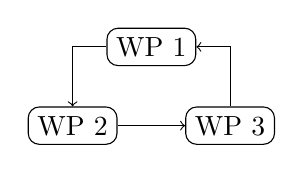
\begin{tikzpicture}
		\draw (0,0) node[draw,rounded corners](WP1) {WP 1};
		\draw (-1, -1) node[draw,rounded corners](WP2) {WP 2};
		\draw (1, -1) node[draw,rounded corners](WP3) {WP 3};
        \draw[->] (WP1) -| (WP2);
        \draw[->] (WP2) -- (WP3);
        \draw[->] (WP3.north) |- (WP1.east);
    \end{tikzpicture}
    \caption{Some diagram representing the relations between the packages.}
    \label{fig:example}
\end{figure}

\lipsum[7]

\begin{table}[!ht]
	\centering
    \begin{tabular}{r r r r}
    	\hline
        \rowcolor{headcolor!20}
    	\textbf{A} & \textbf{B} & \textbf{C} & \textbf{D} \\
    	\hline
        15.99 & 98.98 & 13.67 &  6.25 \\
        16.98 & 65.21 & 63.74 & 25.87 \\
        98.97 &  6.98 & 19.75 & 36.74 \\
        67.39 & 96.84 & 34.14 & 19.85 \\
    	\hline
	\end{tabular}
    \caption{Some example table.}
    \label{tab:example}
\end{table}

\lipsum[8]

\begin{equation}
	y = f(x)
    \label{eq:example}
\end{equation}


%%% WP 0
\wpdef{wp:ProjMgt}{Project Management}
% leader
\textbf{Leaders: \colUGE{A. L'HOSTIS (Univ Eiffel)} \colEFF{M. WENDELN (Efficacity)}}

% description

% Deliverables & co.
\vspace{0.25cm}
\noindent\textbf{Deliverables:} bla bla bla bla.





%%% WP 1
\wpdef{wp:Data}{Drivers for the decarbonation of territories} 
% leader
\textbf{Leader: xxxxxxxxxxxxxx}

% description

\begin{itemize}
    \item état de l’art croisé : approches opérationnelles et scientifiques
    \item hiérarchisation des leviers à « outiller » en priorité (leviers à fort impact GES, où la recherche scientifique a le plus à apporter aux décideurs territoriaux)
    \item \textit{livrable final : }méthode d’évaluation des impacts GES des principaux leviers urbains, s’appuyant sur des outils de modélisation
\end{itemize}


% task
\tdef{tsk:DataST}{some task}


% task
\tdef{tsk:DataOT}{Some other task}


% task
\tdef{tsk:DataLT}{Last task of this WP}


% Deliverables & co.
\vspace{0.25cm}
\noindent\textbf{Deliverables:} some reports.

\noindent\textbf{Success indicators:} scientific publications.

\noindent\textbf{Partners involved:} \colEGS{LMQ}, \colUE{LITA}, \colUT{CGCS}.





%%% WP 2
\wpdef{wp:Classif}{Scenarios}
% leader
\textbf{Leader: xxxxxxxxxxxxxxxxxxx}

% description

\begin{itemize}
    \item Comment concevoir des scénarios de rupture (nécessaires à l’atteinte des objectifs GES des territoires) ? Sur quelles bases ?
    \item Comment les relier aux scénarios opérationnels (utilisés dans la planification et la programmation opérationnelle) ? 
    \item Quels nouveaux outils, modèles et données nécessaires ? 
\end{itemize}

% task
\tdef{tsk:ClassifFT}{First task of this WP}

% task
\tdef{tsk:ClassifAT}{Another task}

% task
\tdef{tsk:ClassifYT}{Yet another task}

% Deliverables & co.
\vspace{0.25cm}
\noindent\textbf{Deliverables:} some reports.

\noindent\textbf{Success indicators:} scientific publications.

\noindent\textbf{Partners involved:} \colINR{LMD}, \colEGS{LMQ}.

%%% WP 3
\wpdef{wp:Exp}{Data?}


\wpdef{wp:Exp}{Implementing models}


\wpdef{wp:Exp}{Other WP?}

Lots 3 à 8 – approfondissements par grandes approches sectorielles : préparation des états de l’art complémentaires, cas d’usage, modèles et données nécessaires

\begin{itemize}
    \item Hypothèses et modèles transverses : hypothèses démographiques et économiques, usage du sol, intégration des données et modèles à différentes échelles spatiales 
    \item Bâtiments et systèmes énergétiques urbains
    \item Transports de personne (tous leviers)
    \item Transports de marchandises (tous leviers)
    \item Référentiel définitif : évaluations carbone, indicateurs complémentaires ; compléments sur les autres secteurs urbains (industrie, déchets, eau…)
\end{itemize}



%%% WP 3
\wpdef{wp:Exp}{Exploiting models results, interaction with territorial stakeholders}
% leader
\textbf{Leader: xxxxxxxxxxxxxxxxxxx}

% description
\begin{itemize}
    \item Une coordination transverse 
    \item Une coordination locale par chaque université sur son territoire d’installation
\end{itemize}

% task
\tdef{tsk:ExpYT}{Yet another task}

% task
\tdef{tsk:ExpTT}{Just two tasks in this WP}

% Deliverables & co.
\vspace{0.25cm}
\noindent\textbf{Deliverables:} some reports.

\noindent\textbf{Success indicators:} scientific publications.

\noindent\textbf{Partners involved:} \colINR{LMD}, \colEGS{LMQ}, \colUE{LITA}, \colTUT{FI}.



\wpdef{wp:Exp}{Valorisation: infusing knowledge, methods, and the practionners toolbox}
% leader
\textbf{Leader: xxxxxxxxxxxxxxxxxxx}
% description
\begin{itemize}
    \item     Production de connaissances scientifiques (publications, colloques, etc.)
    \item Développement des modèles universitaires
    \item Transfert des développements méthodologiques, et des modèles pour enrichir, développer la boîte à outils opérationnels (Efficacity) 
\end{itemize}



%%%
Table~\ref{tab:schedule} shows the list of deliverables of the project, while Figure~\ref{fig:gantt} presents the chronology of the WPs and tasks.

\begin{table}[htb!]
	\centering
	\begin{tabular}{l r l p{8cm} l}
		\hline
        \rowcolor{headcolor!20}
		\textbf{Delivery date} & \textbf{WP} & \textbf{Item} & \textbf{Title} & \textbf{Nature} \\
		\hline
		$t_0$ & \ref{wp:ProjMgt} & WS0 & Project Website & Website \\
		$t_0+3$ & \ref{wp:ProjMgt} & R0.1 & Post-meeting report & Short report \\
		$t_0+9$ & \ref{wp:Data} & W1 & International workshop & Workshop \\
		$t_0+15$ & \ref{wp:ProjMgt} & R0.2 & Post-meeting report & Short report \\
		$t_0+18$ & \ref{wp:Data} & W2 & Great symposium & Workshop \\
		$t_0+21$ & \ref{wp:Data} & R1.1 & Mid-term report on the data & Technical report \\
		$t_0+21$ & \ref{wp:Classif} & R2.1 & Mid-term report on the classification methods & Technical report \\
		$t_0+21$ & \ref{wp:Classif} & R2.2 & Mid-term report on the experiments & Technical report \\
		$t_0+24$ & \ref{wp:ProjMgt} & R0.3 & Post-meeting report & Short report \\
		$t_0+33$ & \ref{wp:Classif} & AP1 & Tool prototype & Software \\
		$t_0+36$ & \ref{wp:Exp} & WS1 & Finalized tool and Webapp & Software \\
		$t_0+36$ & \ref{wp:Exp} & R3.1 & Documentation of the software & Technical report \\
		$t_0+36$ & \ref{wp:Exp} & R3.2 & Final report & Technical report \\
		\hline
	\end{tabular}
	\caption{Task Schedule of the project.}
    \label{tab:schedule}
\end{table}
\noteANR{\textbf{Non-ANR} note: this table does not seem to be required anymore. But it can be useful, let us keep it for now.}

\begin{figure}[!ht]
	\centering
    \begin{ganttchart}[time slot format=isodate-yearmonth, 
		vgrid={dotted,draw=none,draw=none}, %hgrid=true, 
		x unit=0.35cm,									% NOTE: width for a single month
		y unit chart = 0.6cm, bar height=0.6,
		y unit title = 0.5cm, title height=1,
		include title in canvas=false,
        time slot unit=month
	%]{2018-09}{2021-10}
	]{2018-09}{2022-02}
    
	% temporal marks
	\gantttitlecalendar[title/.style={fill=black!30,draw=black}]{year} \\
	\gantttitlecalendar[title/.style={fill=black!20,draw=black}]{month} \\
    
	% horizontal bars
 	\ganttbarbis{WP~\ref{wp:ProjMgt}}{Projet coordination}{2018-10}{2021-07}{blue!50} \\
    
 	\ganttbarbis{WP~\ref{wp:Data}}{Data retrieval}{2018-10}{2020-07}{red!50} \\
 	\ganttbarbis{Task~\ref{tsk:DataST}}{Some task}{2018-10}{2019-02}{red!25} \\
 	\ganttbarbis{Task~\ref{tsk:DataOT}}{Some other task}{2018-10}{2019-08}{red!25} \\
 	\ganttbarbis{Task~\ref{tsk:DataLT}}{Last task of this WP}{2019-03}{2020-07}{red!25} \\
    
 	\ganttbarbis{WP~\ref{wp:Classif}}{Classification methods}{2018-10}{2020-08}{green!50} \\
 	\ganttbarbis{Task~\ref{tsk:ClassifFT}}{First task of this WP}{2018-10}{2020-08}{green!25} \\
 	\ganttbarbis{Task~\ref{tsk:ClassifAT}}{Another task}{2019-03}{2019-10}{green!25} \\
 	\ganttbarbis{Task~\ref{tsk:ClassifYT}}{Yet another task}{2019-11}{2020-07}{green!25} \\
    
 	\ganttbarbis{WP~\ref{wp:Exp}}{Experimental validation}{2019-03}{2021-08}{purple!50} \\
 	\ganttbarbis{Task~\ref{tsk:ExpYT}}{Yet another task}{2019-03}{2020-12}{purple!25} \\
 	\ganttbarbis{Task~\ref{tsk:ExpTT}}{Just two tasks in this WP}{2021-01}{2021-09}{purple!25} \\
    
	% items
 	\ganttmilestone{Items}{2018-10}
 	\ganttmilestone{}{2019-01}
 	\ganttmilestone{}{2019-07}
 	\ganttmilestone{}{2020-01}
 	\ganttmilestone{}{2020-04}
 	\ganttmilestone{}{2020-07}
 	\ganttmilestone{}{2020-10}
	\ganttmilestone{}{2021-07}
 	\ganttmilestone{}{2021-09}
    
	% vertical lines
% 	\drawverticalline{2019-11}{xxxxx}
% 	\drawverticalline{2020-01}{yyyyy}
\end{ganttchart}

	\caption{Gantt Diagram of the project.}
    \label{fig:gantt}
\end{figure}














%%%%%%%%%%%%%%%%%%%%%%%%%%%%%%%%%%%%%%%%%%%%%%%%%%
%%%%%%%%%%%%%%%%%%%%%%%%%%%%%%%%%%%%%%%%%%%%%%%%%%
\section{Project organisation and management}

%%%%%%%%%%%%%%%%%%%%%%%%
\subsection{Project manager}
\notePEPR{Fournir les éléments permettant d’évaluer la capacité du Responsable du projet à piloter et coordonner le projet1. CV du responsable du projet (section 8) : il est vivement conseillé aux candidats de rédiger leur CV en anglais et de ne pas utiliser d'abréviations car les évaluations peuvent être effectuées par des non francophones.}

\subsection{Organization of the partnership}
\notePEPR{Présenter les éléments permettant d’apprécier la qualité du groupement. Décrire les compétences et la qualité des entités mobilisées dans le cadre du projet. Les éléments d’appréciation du groupement peuvent être des réalisations passées, des indicateurs (publications), l’adéquation de l’engagement scientifique de l’entité par rapport aux objectifs du PEPR, les infrastructures dont elle dispose ou auxquelles elle a accès, etc.}
\notePEPR{Présenter les postes clés du projet, par exemple les responsables d’un lot. La granularité du détail devra être ajustée à l’ampleur du projet. Typiquement, 3 à 6 personnes peuvent être décrites. Une liste des autres acteurs importants peut être donnée.}
\notePEPR{Préciser pour chacun des partenaires (parties prenantes), sa contribution, son apport autour de ses métiers et ses pratiques (compléter le tableau « métiers et pratiques » – annexe partenariats).}
\notePEPR{Précisez pour les laboratoires non financés (Européens, Internationaux), leur contribution et leur apport dans le projet ainsi que leur rôle dans la réalisation des objectifs (compléter le tableau « laboratoires non financés » – annexe partenariats).}
\notePEPR{Présenter les terrains envisagés afin d’ancrer les recherches proposées sur un territoire (compléter le tableau « terrains envisagés » – annexe partenariats).}
\notePEPR{Montrer la complémentarité des partenaires du consortium au regard des objectifs du projet et la valeur ajoutée apportée par chaque entité.}

\subsection{Management framework}
\notePEPR{Préciser l’organisation entre partenaires, ainsi que les modalités de pilotage du projet.}
\notePEPR{Définir la méthode de suivi des indicateurs et des jalons. Décrire la façon dont seront gérés les différents risques anticipés pour le projet.}
\notePEPR{Préciser les modalités d’accès aux ressources partagées, de valorisation des résultats, et de partage de la propriété intellectuelle et industrielle.}
\notePEPR{Indiquer précisément le lien avec le pilotage global du PEPR et l’intégration dans ses outils de suivi.}
\notePEPR{Indiquer précisément le lien avec les centres opérationnels et les mises en synergie proposées ; expliciter, si c’est nécessaire les complémentarités avec d’autres projets déposés dans le même appel ou dans d’autres appels.}

\subsection{Institutional strategy}
\notePEPR{Décrire comment le projet s’inscrit dans la stratégie des établissements partenaires et comment les établissements soutiennent le projet dans sa durée. Décrire quels sont les principaux moyens et dispositifs mis à disposition par les établissements au projet.}
\notePEPR{Indiquez comment le projet participe à l’animation de la communauté VDBI à une échelle nationale en impliquant les établissements participants, laboratoires et partenaires.}




\begin{table}[h]
	\centering
    \small
    \begin{tabular}{p{0.10\textwidth} p{0.13\textwidth} p{0.24\linewidth} p{0.14\linewidth} p{0.11\linewidth} p{0.12\linewidth}}
		\hline
        \rowcolor{headcolor!20}
	    \textbf{Researcher} & \textbf{Person.month} & \textbf{Call, funding agency, \newline grant allocated} & \textbf{Project's title} & \textbf{Scientific \newline coordinator} & \textbf{Start--End} \\
		\hline
		... & ... & ... & ... & ... & ... \\
		... & ... & ... & ... & ... & ... \\
		\hline
	\end{tabular}
	\caption{Implication of the scientific coordinator and partner's scientific leader in on-going project(s)}
\end{table}



\begin{table}[h]
	\centering
    \small
    \begin{tabular}{p{0.10\textwidth} p{0.13\textwidth} p{0.24\linewidth} p{0.14\linewidth} p{0.11\linewidth} p{0.12\linewidth}}
		\hline
        \rowcolor{headcolor!20}
	    \textbf{Researcher} & \textbf{Person.month} & \textbf{Call, funding agency, \newline grant allocated} & \textbf{Project's title} & \textbf{Scientific \newline coordinator} & \textbf{Start--End} \\
		\hline
		... & ... & ... & ... & ... & ... \\
		... & ... & ... & ... & ... & ... \\
		\hline
	\end{tabular}
	\caption{Implication of the scientific coordinator in on-going project(s)}
\end{table}

The project \textsc{MyProJecT} is coordinated by \colUE{Stéphanie MARTIN (LITA)}. It is organized in four technical WPs divided in tasks. Each WP is under the responsibility of a well-identified coordinator namely \colUE{Stéphanie MARTIN (LITA)} for WP~\ref{wp:ProjMgt}, \colEGS{Jing ZANG (LMQ)} for WP~\ref{wp:Data}, \colINR{Assa DIALA (LMD)} for WP~\ref{wp:Classif}, and \colINR{Richard MEUNIER (LMD)} for WP~\ref{wp:Exp}.

%%%
\paragraph*{\colUE{S. MARTIN}} \hspace{-1em} is blablabla at the \colUE{Laboratoire d'Informatique Théorique et Appliquée} with Université de l'excellence. \lipsum[7] 

Beside the coordination (WP~\ref{wp:ProjMgt}), she will be involved in WP~\ref{wp:Data}, \ref{wp:Classif} and \ref{wp:Exp}.

%%%
\paragraph*{\colEGS{J. ZANG}} \hspace{-1em} is the leader of WP 1. He is bla bla bla at the \colEGS{Laboratoire de Métaphysique Quantique} with École générale supérieure. \lipsum[2] 

He will participate in all tasks of WP~\ref{wp:Data}.

%%%
\paragraph*{\colINR{A. DIALA}} \hspace{-1em} is the leader of WP~\ref{wp:Classif}. She is bla bla bla at the \colINR{Laboratoire de Mathématiques très Discrètes} with Institut national de la recherche. \lipsum[8] 

He will work on several tasks of WP~\ref{wp:Classif}.

%%%
\paragraph*{\colINR{R. MEUNIER}} \hspace{-1em} is the leader of WP~\ref{wp:Exp}. He is bla bla bla at the \colINR{Laboratoire de Mathématiques très Discrètes} with Institut national de la recherche. \lipsum[9]

He will work on WP~\ref{wp:Classif} and \ref{wp:Exp}.

%%%
\paragraph*{Other project members:} \colEGS{A.~MANSOURI} (Professor at \colEGS{Laboratoire de Métaphysique Quantique} with École générale supérieure), he has a strong expertise in bla bla bla bla. He will be involved in Tasks~\ref{tsk:ExpYT} and \ref{tsk:ExpTT}.

\colUE{R. GONZALES} (Associate Professor at the \colUE{Laboratoire d'Informatique Théorique et Appliquée} with the Université de l'excellence), he is specialized in bla bla bla. He will participate in Tasks~\ref{tsk:ExpYT} and \ref{tsk:ExpTT}.

\colUT{D. WAKEFIELD} (Assistant Professor at the \colUT{Center for Great Computer Science} with the University of Tadborough), a specialist of blablabla bla blabla blabla. She will take part in Tasks~\ref{tsk:DataOT} and \ref{tsk:DataLT}.
.

\colTUT{O. MÜLLER} (Professor at the \colTUT{Forschungszentrum für Informatik} with Technische Universität Turmstadt), he works on bla bla bla bla. He will participate in Tasks~\ref{tsk:ExpYT} and \ref{tsk:ExpTT}.




%%%%%%%%%%%%%%%%%%%%%%%%










%%%%%%%%%%%%%%%%%%%%%%%%%%%%%%%%%%%%%%%%%%%%%%%%%%
%%%%%%%%%%%%%%%%%%%%%%%%%%%%%%%%%%%%%%%%%%%%%%%%%%
\section{Expected outcomes of the project}
\notePEPR{Décrire les résultats scientifiques attendus, ainsi que leurs impacts potentiels dans le domaine du PEPR. }
\notePEPR{Décrire comment les résultats scientifiques s’inscrivent dans une trajectoire de transformation globale socio-économique-technique-écologique-territorial ; en quoi ces résultats scientifiques sont-ils transformants et transposables pour assurer les transformations nécessaires des Villes et bâtiments en villes et bâtiments durables.}
\notePEPR{Détailler la stratégie de diffusion et de valorisation des résultats, y compris les actions de promotion de la culture scientifique. Décrire comment le projet envisage de promouvoir les résultats de la recherche auprès des autorités publiques concernées (État, collectivités, agences) et auprès du grand public.}
\notePEPR{Préciser finement comment le projet nourrira le reste du PEPR et le reste de la stratégie nationale.}
\notePEPR{Décrire finement comment les résultats du projet pourront être réutilisés par la communauté (codes, connaissances, données, préconisations, retours d’expériences, ...) permettant de proposer des solutions pour une Ville Durable et Bâtiment Innovant.}
\notePEPR{Expliquer la stratégie de préparation et de diffusion des résultats et données liées au projet.}
\notePEPR{Préciser les retombées à court terme (pour des expérimentations lancées pendant le projet) ou à moyen terme (pour des expérimentations issues du projet).}


\section{Funding justification}
\notePEPR{Indiquer les détails des moyens matériels, financiers et humains, qui seront mobilisés dans le cadre du projet et leur adéquation par rapport aux objectifs. L’établissement coordinateur justifiera les moyens qu’il demande au titre de l’ensemble du consortium, sur la durée du projet, en indiquant les mécanismes qu’il mettra en œuvre pour distribuer ces moyens ainsi que ceux mis à disposition par les partenaires du projet, ou ceux qui seront obtenus en cofinancement. Les dépenses éligibles (décrites dans le Règlement Financier) doivent avoir un lien direct avec les actions de recherche du projet.}

\begin{comment}

% exemple de table reprise du template unofficial ANR
\begin{table}[h]
	\centering
    \small
	\begin{tabular}{p{0.31\textwidth} r r r r r}
		\hline
        \rowcolor{headcolor!20}
	    & \textbf{Partner} & \textbf{Partner} & \textbf{Partner} & \textbf{Partner} & \textbf{Partner} \\
        \rowcolor{headcolor!20}
	    & \textbf{\colUE{LITA (UE)}} & \textbf{\colEGS{LMQ (EGS)}} & \textbf{\newline\colINR{LMD (INR)}} & \textbf{\newline\colUT{CGCS (UT)}} & \textbf{\newline\colTUT{FI (TUT)}} \\
		\hline
		Staff expenses & 250~000\euro & 100~000\euro & 200~000\euro & 75~000\euro & 100~000\euro \\
		Instruments and material costs & 5~000\euro & 7~500\euro & 3~000\euro & 9~000\euro & 6~000\euro \\
		Building and ground costs & 3~000\euro & 98~000\euro & 0\euro & 0\euro & 0\euro \\
		Outsourcing / subcontracting & 0\euro & 0\euro & 0\euro & 11~000\euro & 7~000\euro \\
		Overheads costs\footnote{including missions expenses, general and administrative costs \& other operating expenses} & 8~000\euro & 6~500\euro & 12~345\euro & 5~000\euro & 11~000\euro \\
		Administrative management \& structure costs & 100\euro & 10\euro & 150\euro & 30\euro & 2\euro \\
		\hline
        \rowcolor{headcolor!20}
		\textbf{Sub-total} & \textbf{266~100\euro} & \textbf{212~010\euro} & \textbf{215~495\euro} & \textbf{100~030\euro} & \textbf{124~002\euro} \\
		\hline
        \rowcolor{headcolor!40}
		\textbf{Requested} & \multicolumn{5}{c}{\textbf{917~637\euro}} \\
		\hline
	\end{tabular}
	\caption{Requested means by item of expenditure and by partner.}
\end{table}

\end{comment}






%%%%%%%%%%%%%%%%%%%%%%%%%%%%%%%%%%%%%%%%%%%%%%%%%%
\section{Cited references}

\notePEPR{Lister les références bibliographiques citées dans le document scientifique du projet (souligner les noms des partenaires du consortium lorsqu’ils sont auteurs) (Quatre pages maximum).}

\textbf{Note}: names of authors who belong to the consortium are displayed in \textbf{bold}.

% derived from https://tex.stackexchange.com/questions/73136/make-specific-author-bold-using-biblatex/73246#73246
\renewcommand*{\boldnames}{}
%\forcsvlist{\listadd\boldnames}
%  {{Herrmann, Wolfgang~A.}, {Herrmann, W.~A.}, {Herrmann, Wolfgang\bibnamedelima A.},
%   {Herrmann, W\bibinitperiod\bibinitdelim A\bibinitperiod}}
\forcsvlist{\listadd\boldnames}
  {{Kilani, Moez}, {Kilani, M.}, {Kilani, M\bibinitperiod}}
\forcsvlist{\listadd\boldnames}
  {{Zerguini, Seghir}, {Zerguini, S.}, {Zerguini, S\bibinitperiod}}
\forcsvlist{\listadd\boldnames}
  {{L'Hostis, Alain}, {L'Hostis, A.}, {L'Hostis, A\bibinitperiod}}
\forcsvlist{\listadd\boldnames}
  {{Liu, Liu}, {Liu, L.}, {Liu, L\bibinitperiod}}
  \forcsvlist{\listadd\boldnames}
  {{Manout, Ouassim}, {Manout, O.}, {Manout, O\bibinitperiod}}


{	\setstretch{0.8}							% decreases the space between lines
	\phantomsection
	\addcontentsline{toc}{section}{References}	% add bibliography to toc
	\printbibliography[heading=none]							% add the references
}

\section{Linked projects}
\notePEPR{Lister et décrire les projets en cours de financement, liés au projet présenté. La description de chaque projet doit résumer l’objectif final, l’état de l’art, les grandes étapes de réalisation avec les principales techniques utilisées et la place des différentes partenaires dans leur réalisation (Deux pages maximum). }

\section{Project leader CV}
\notePEPR{CV du responsable du projet : il est vivement conseillé aux candidats de rédiger leur CV en anglais et de ne pas utiliser d'abréviations car les évaluations peuvent être effectuées par des non francophones.}


\appendix{}

\section{Stakeholders Appendix}
\notePEPR{La section ci-dessous, constitué de l’Annexe Partenariats et de l’Annexe Publications, ne doit pas dépasser les 10 pages. }
\notePEPR{Dans cette annexe, 
    • préciser pour chacun des partenaires de type partie prenante, sa contribution, son apport autour de ses métiers et ses pratiques }
\notePEPR{précisez pour les laboratoires non financés (Européens, Internationaux), leur contribution et leur apport dans le projet ainsi que leur rôle dans la réalisation des objectifs}
\notePEPR{présenter les terrains envisagés afin d’ancrer les recherches proposées sur un territoire}




{	\vspace{0.2cm}
	\centering
    \small
    \begin{table}
        \begin{tabular}{p{0.15\textwidth} p{0.20\textwidth} p{0.45\linewidth} } 
        \hline 
        \rowcolor{headcolor!20}
        \textbf{Métiers et pratiques / Domain and practices}& \textbf{Noms – Prénoms / Name – First name}& \textbf{Partie-Prenante /  Stakeholders}\\ \hline 
             &  & \\ \hline 
             &  & \\ \hline 
             &  & \\ \hline 
             &  & \\ \hline
        \end{tabular}
        \caption{Domain and practice}
        \label{tab:my_label}
    \end{table}
}    
{	\vspace{0.2cm}
	\centering
    \small
    \begin{table}
        \centering
        \begin{tabular}{p{0.15\textwidth} p{0.25\textwidth} p{0.15\linewidth} p{0.20\linewidth}  p{0.15\textwidth}  p{0.05\textwidth}}
        \hline 
        \rowcolor{headcolor!20}
        \textbf{Discipline / subject}& \textbf{Noms – Prénoms- Orcid1 des personnes/ Name – First name - Orcid}& \textbf{Laboratoire/ Laboratory}& \textbf{Etablissement de rattachement des personnes/ Person's home establishment}& \textbf{Pays/ Country} &\\ \hline 
              &&  &  &\\ \hline 
              &&  &  &\\ \hline 
              &&  &  &\\ \hline 
              &&  &  &\\ \hline
        \end{tabular}
        \caption{Not funded laboratories / Laboratoires non financés}
        \label{tab:my_label}
    \end{table}
}    


{	\vspace{0.2cm}
	\centering
    \small
    \begin{table}
        \centering
        \begin{tabular}{p{0.15\textwidth} p{0.20\textwidth} p{0.45\linewidth} p{0.15\linewidth} }
		\hline
        \rowcolor{headcolor!20}
	    \textbf{Terrain/ Site}& \textbf{Noms – Prénoms- du porteur territorial/ Territorial carrier Name – First name}& \textbf{Expérimentation envisagée ou déjà lancée/ Experiments planned or already launched}& \textbf{Inscrit dans un dispositif aidé par la Banque des Territoires (DVD, TID…)/ Part of a scheme supported by the Banque des Territoires}\\	\hline
        & & & \\ \hline
		& & & \\ \hline
		& & & \\ \hline
	\end{tabular}
    \caption{Envisaged territories / Terrains envisagés}
    \label{tab:my_label}
    \end{table}

}

\section{Publications Appendix}
\notePEPR{Dans cette annexe, chaque entité indiquera la liste de ses publications des 3 dernières années (2021-2023). 
Cette liste peut intégrer des publications à destination des utilisateurs des résultats de la recherche (presse professionnelle, etc…) en les distinguant des publications dans des revues scientifiques à comité de lecture. 
La liste peut aussi intégrer des pre-prints non encore publiés dans des journaux scientifiques avec comité de lecture, en particulier pour le référencement de données préliminaires. Si disponibles, indiquez les liens open-access des références pour améliorer leur accessibilité aux évaluateurs. Surligner les noms des auteurs/co-auteurs participant au projet.}

\end{document}




%%%%%%%%%%%%%%%%%%%%%%%%%%%%%%%%%%%%%%%%%%%%%%%%%%
%%%%%%%%%%%%%%%%%%%%%%%%%%%%%%%%%%%%%%%%%%%%%%%%%%
%%%%%%%%%%%%%%%%%%%%%%%%%%%%%%%%%%%%%%%%%%%%%%%%%%
% TODO
% garder les sections* dans les liens du PDF
